\let\negmedspace\undefined
\let\negthickspace\undefined
\documentclass[journal]{IEEEtran}
\usepackage[a5paper, margin=10mm, onecolumn]{geometry}
%\usepackage{lmodern} % Ensure lmodern is loaded for pdflatex
% \usepackage{tfrupee} % Include tfrupee package

\setlength{\headheight}{1cm} % Set the height of the header box
\setlength{\headsep}{0mm}     % Set the distance between the header box and the top of the text

\usepackage{gvv-book}
\usepackage{gvv}
\usepackage{cite}
\usepackage{amsmath,amssymb,amsfonts,amsthm}
\usepackage{algorithm}
\usepackage{algorithmic}
\usepackage{graphicx}
\usepackage{textcomp}
\usepackage{xcolor}
\usepackage{txfonts}
\usepackage{listings}
\usepackage{enumitem}
\usepackage{mathtools}
\usepackage{gensymb}
\usepackage{comment}
\usepackage[breaklinks=true]{hyperref}
\usepackage{tkz-euclide} 
\usepackage{listings}
% \usepackage{gvv}                                        
\def\inputGnumericTable{}                                 
\usepackage[latin1]{inputenc}                                
\usepackage{color}                                            
\usepackage{array}                                            
\usepackage{longtable}                                       
\usepackage{calc}                                             
\usepackage{multirow}                                         
\usepackage{hhline}                                           
\usepackage{ifthen}                                           
\usepackage{lscape}
% \usepackage{algpseudocode}
\begin{document}

\bibliographystyle{IEEEtran}
\vspace{3cm}

\title{NCERT 10.4.3.6}
\author{EE24BTECH11053 - S A Aravind Eswar}
% \maketitle
% \newpage
% \bigskip
{\let\newpage\relax\maketitle}

\renewcommand{\thefigure}{\theenumi}
\renewcommand{\thetable}{\theenumi}
\setlength{\intextsep}{10pt} % Space between text and floats

\textbf{Question:} A letter is chosen in random from the word 'ASSASSINATION'. Find the probability that the letter chosen is
\begin{enumerate}
    \item A vowel
    \item A consonant
\end{enumerate}

\section{Theoretical solution}
    Taking vowel as 1 and consonant as 0,

    We can count and conclude that,

    The Bernoulli's random variable's PMF as,
    % And PMF of the above random variable as,
    \begin{align}
        f_X(n) = \begin{cases}
            \frac{6}{13},& n=0\\
            \frac{7}{13},& n=1\\
            0,& \text{otherwise}
        \end{cases}
    \end{align}

    And the CDF of it is,

    \begin{align}
        C_X(n) = \begin{cases}
            0,& n<0\\
            \frac{6}{13},& 0\leq n<1\\
            1,&n\geq1
        \end{cases}
    \end{align}

    Thus the probability to get a vowel is $\frac{6}{13}$ and a consonant is $\frac{7}{13}$
\section{Numberical Solution}
    We will use the Monte Carlo method to estimate the probability.

    First to choose a random number, we have to make a pseudo-random number generator, as it is not possible for computers to produce true randomness

    A commonly used RNG(Random Number Generator) is Linear Congruential Generator(LCG). It's given by the following reccurrence relation,
    \begin{align}
        X_{n+1} = \brak{aX_n+c}\text{mod}\,m
    \end{align}
    where,
    \begin{align}
        m,\,& 0<m<1&\dashcolon \text{the "modulus"}\\
        a,\,& 0<a<m&\dashcolon\text{the "multiplier"}\\
        c,\,& 0\leq c<m&\dashcolon\text{the "increment"}\\
        X_0\,&0\leq X_0<m&\dashcolon\text{the "seed" or "start value"}
    \end{align}

    This algorithm is really useful for general generation of random number as it uses less memory. But it cannot be used for cryptographic encryption because it's simple to crack it.
    But we wouldn't need any further complex RNGs as this will suffice for this.

    \begin{figure}[H]  
        \centering  
        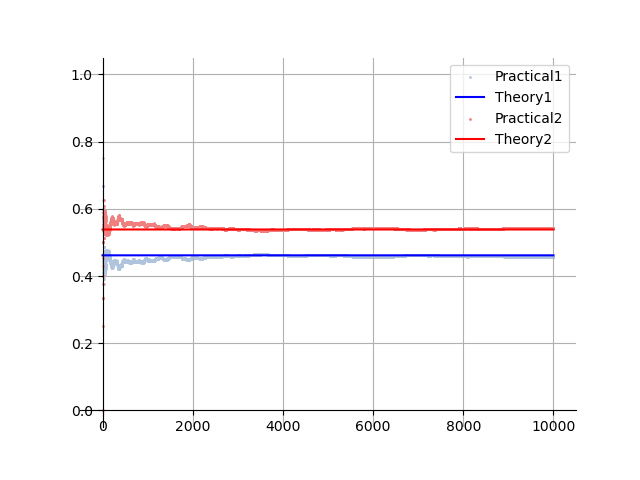
\includegraphics[width=\columnwidth]{figs/fig1.png}  
        \caption{Verification}
        % \columnwidth
    \end{figure}
    \begin{figure}[H]
        \centering
        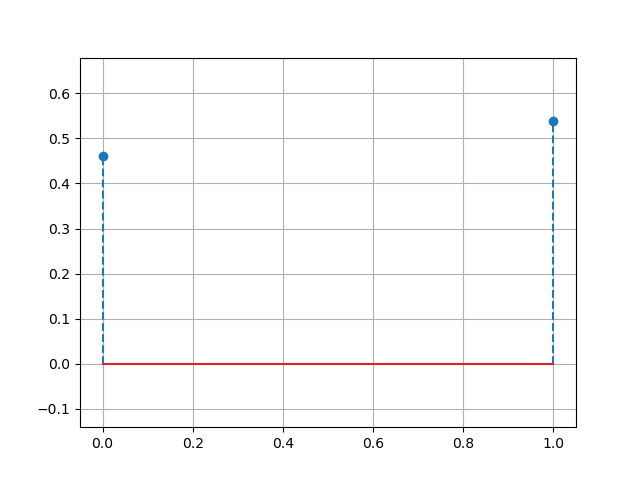
\includegraphics[width=\columnwidth]{figs/fig2.png}
        \caption{Stem Plot}
    \end{figure}
\end{document}
